\section{Analisi dei Risultati}
\label{sec:analisi_risultati}

Questa sezione presenta i risultati quantitativi estratti dall'analisi spaziale delle traiettorie generative. La Tabella \ref{tab:risultati_metriche} riassume le metriche fondamentali discusse nel capitolo precedente per descrivere la struttura dello spazio latente: la qualità della riduzione dimensionale (\textit{Trustworthiness}) e il grado di compattezza e separazione dei cluster (\textit{Silhouette Score}).

\begin{table}[htbp]
\centering
\begin{tabular}{lcc}
\hline
\textbf{Tecnica di Prompting} & \textbf{Trustworthiness} & \textbf{Silhouette Score} \\
\hline
Persona Prompting & 0.934 & 0.466 \\
Few-shot Prompting & 0.936 & 0.536 \\
Chain-of-Thought (CoT) & 0.966 & 0.743 \\
Step-back Prompting & 0.959 & 0.412 \\
Prompt Chaining & 0.959 & 0.484 \\
Tree of Thoughts & 0.967 & 0.520 \\
\hline
\end{tabular}
\caption{Riepilogo delle metriche quantitative estratte dalle traiettorie degli hidden states per le sei tecniche di prompting analizzate.}
\label{tab:risultati_metriche}
\end{table}

\subsubsection*{Affidabilità della proiezione tridimensionale}
I valori di \textit{Trustworthiness} si attestano uniformemente su livelli molto alti, compresi tra 0.934 e 0.967. Questo indicatore conferma che la riduzione dimensionale da 4096 a 3 dimensioni, effettuata tramite l'algoritmo UMAP, preserva in modo fedele la topologia locale e le relazioni di vicinanza tra gli \textit{hidden states} originali. Valori così prossimi a 1 indicano che le traiettorie generative e i cluster osservati nello spazio ridotto sono rappresentazioni matematicamente solide delle reali dinamiche interne del modello linguistico, validando l'intero impianto visivo e analitico della pipeline sperimentale. In particolare, le tecniche che inducono percorsi argomentativi complessi, come il \textit{Chain-of-Thought} e il \textit{Tree of Thoughts}, registrano i livelli massimi di affidabilità (0.966 e 0.967), segnalando che le strutture ramificate o sequenziali mantengono un'alta coerenza topologica.

\subsubsection*{Compattezza e separazione dei domini semantici}
L'analisi del \textit{Silhouette Score} rivela come la struttura sintattica e semantica del prompt influisca direttamente sulla densità e sulla separazione dei raggruppamenti (cluster) formati nello spazio vettoriale.

Il dato più rilevante emerge dalla tecnica \textit{Chain-of-Thought}, che registra il valore di silhouette più elevato in assoluto (0.743). Questo risultato suggerisce che forzare il modello a esplicitare una sequenza di deduzioni logiche produce traiettorie estremamente coese e isolate dal resto dello spazio latente. Il ``tunnel cognitivo'' indotto dal ragionamento passo-passo riduce al minimo il rumore concettuale tra i cluster, mantenendo il modello focalizzato su un'area semantica ad alta densità.

Valori intermedi e indicativi di una buona struttura spaziale si osservano per il \textit{Few-shot Prompting} (0.536) e il \textit{Tree of Thoughts} (0.520). Nel primo caso, l'imposizione di schemi rigorosi e predefiniti (come la formattazione JSON) guida il modello nella creazione di confini netti tra le componenti strutturali dell'output. Nel secondo, l'articolazione in rami decisionali e valutativi genera una segmentazione chiara delle aree semantiche esplorate in ogni singola fase dell'albero concettuale. Il \textit{Prompt Chaining} e il \textit{Persona Prompting} presentano valori leggermente inferiori (rispettivamente 0.484 e 0.466) ma comunque rappresentativi di una clusterizzazione valida e non casuale.

Al contrario, lo \textit{Step-back Prompting} presenta il valore di silhouette più basso tra le tecniche esaminate (0.412). Questo comportamento spaziale trova una giustificazione nella natura stessa della tecnica: il passaggio da una dimensione di astrazione generale a un'applicazione concreta tende a creare traiettorie più diffuse, in cui i concetti teorici sfumano in modo più fluido nelle indicazioni pratiche, generando raggruppamenti concettuali con confini meno marcati e maggiore compenetrazione.

\subsubsection*{Divergenza Semantica}
La Tabella \ref{tab:divergence_summary} riassume la percentuale di volume spaziale esplorata dalle varianti strutturate e non attraversata dalla traiettoria del \textit{bad prompt}. Per le tecniche che prevedono passaggi multipli o ramificati è riportato il valore medio calcolato su tutte le fasi della generazione.

\begin{table}[htbp]
\centering
\begin{tabular}{lc}
\hline
\textbf{Tecnica di Prompting} & \textbf{Divergenza Media (\%)} \\
\hline
Persona Prompting & 85.7\% \\
Few-shot Prompting & 96.3\% \\
Chain-of-Thought (CoT) & 95.2\% \\
Step-back Prompting & 80.4\% \\
Prompt Chaining & 92.2\% \\
Tree of Thoughts & 90.3\% \\
\hline
\end{tabular}
\caption{Sintesi della Divergenza Semantica. Per le tecniche sequenziali o ramificate è indicato il valore medio di divergenza rispetto al prompt di controllo.}
\label{tab:divergence_summary}
\end{table}

I dati indicano che le tecniche di prompting introducono uno scostamento semantico misurabile: in ogni scenario analizzato, il modello genera token in regioni vettoriali diverse rispetto alla richiesta di base, con valori medi superiori all'80\%. Le modifiche strutturali al formato di output (come nel \textit{Few-shot Prompting}) o l'esplicitazione dei passaggi logici (come nel \textit{Chain-of-Thought}) registrano le divergenze maggiori, attestandosi sopra il 95\%. Le tecniche sequenziali presentano valori medi leggermente inferiori, riflettendo la presenza di fasi di ritorno o ancoraggio alle entità del problema originario previste dalle rispettive architetture.

\subsubsection*{Attivazione Concettuale}
Gli spostamenti volumetrici si riflettono sulla ripartizione dei token generati tra i diversi argomenti latenti individuati dall'algoritmo HDBSCAN. Di seguito si analizzano i profili di attivazione di tre tecniche, utili per osservare come il prompt modifichi la distribuzione semantica del modello in presenza di vincoli di formato o scomposizioni del task.

\newpage

\begin{figure}[htbp]
    \centering
    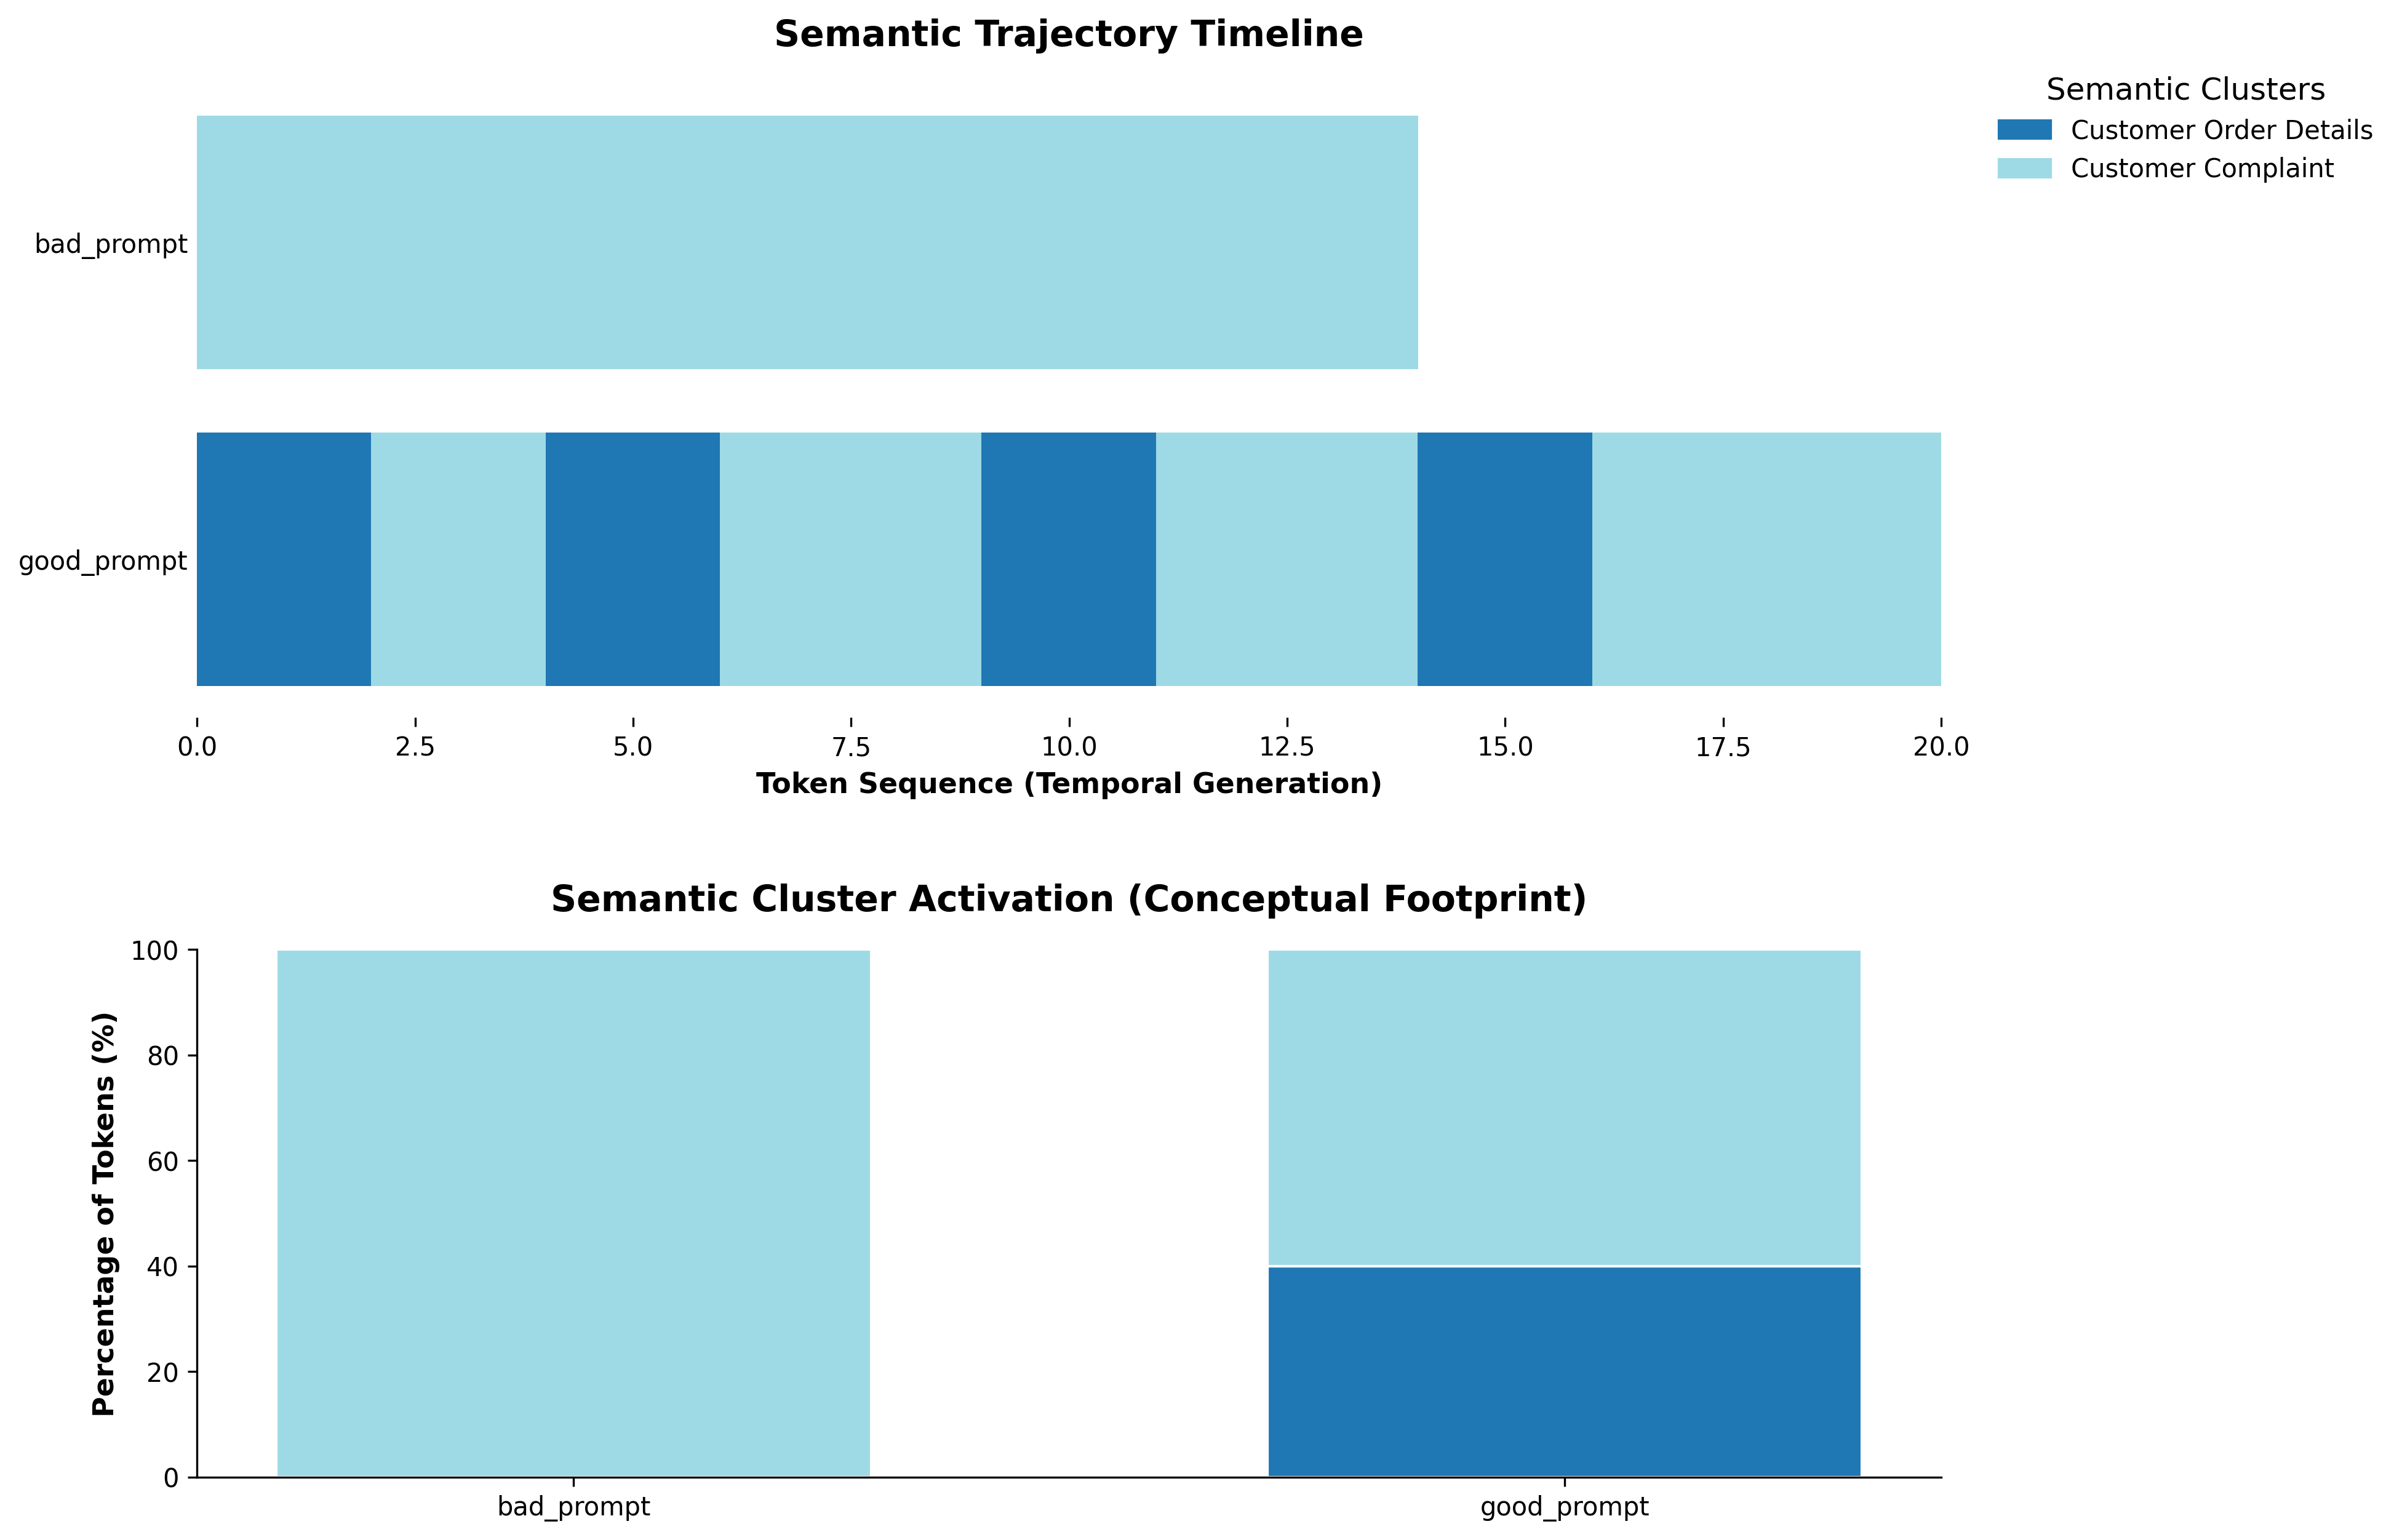
\includegraphics[width=1\textwidth]{assets/few-shot-prompting_cluster_activation.png}
    \caption{Cluster Activation nel Few-shot Prompting. Si osserva una ripartizione tra due cluster principali.}
    \label{fig:act_fewshot}
\end{figure}

\paragraph{Biforcazione Strutturale: Few-shot Prompting}
L'introduzione di esempi formattati produce un cambiamento nella distribuzione dei cluster associato al vincolo di output.

Mentre il \textit{bad prompt} alloca la totalità dei token in un singolo cluster (coerentemente con una generazione puramente discorsiva), il \textit{few-shot prompt} ripartisce l'attivazione principalmente su due cluster (40\% e 60\%), come mostrato in Figura \ref{fig:act_fewshot}. Questa distribuzione riflette la struttura del task richiesto, caratterizzato dall'alternanza tra la produzione della sintassi del formato JSON (chiavi e parentesi) e l'effettiva estrazione del contenuto testuale dal contesto.

\paragraph{Transizione Sequenziale: Prompt Chaining}
Nel Prompt Chaining, la scomposizione del compito in sotto-unità porta il modello ad attraversare in sequenza cluster semantici distinti.

\begin{figure}[htbp]
    \centering
    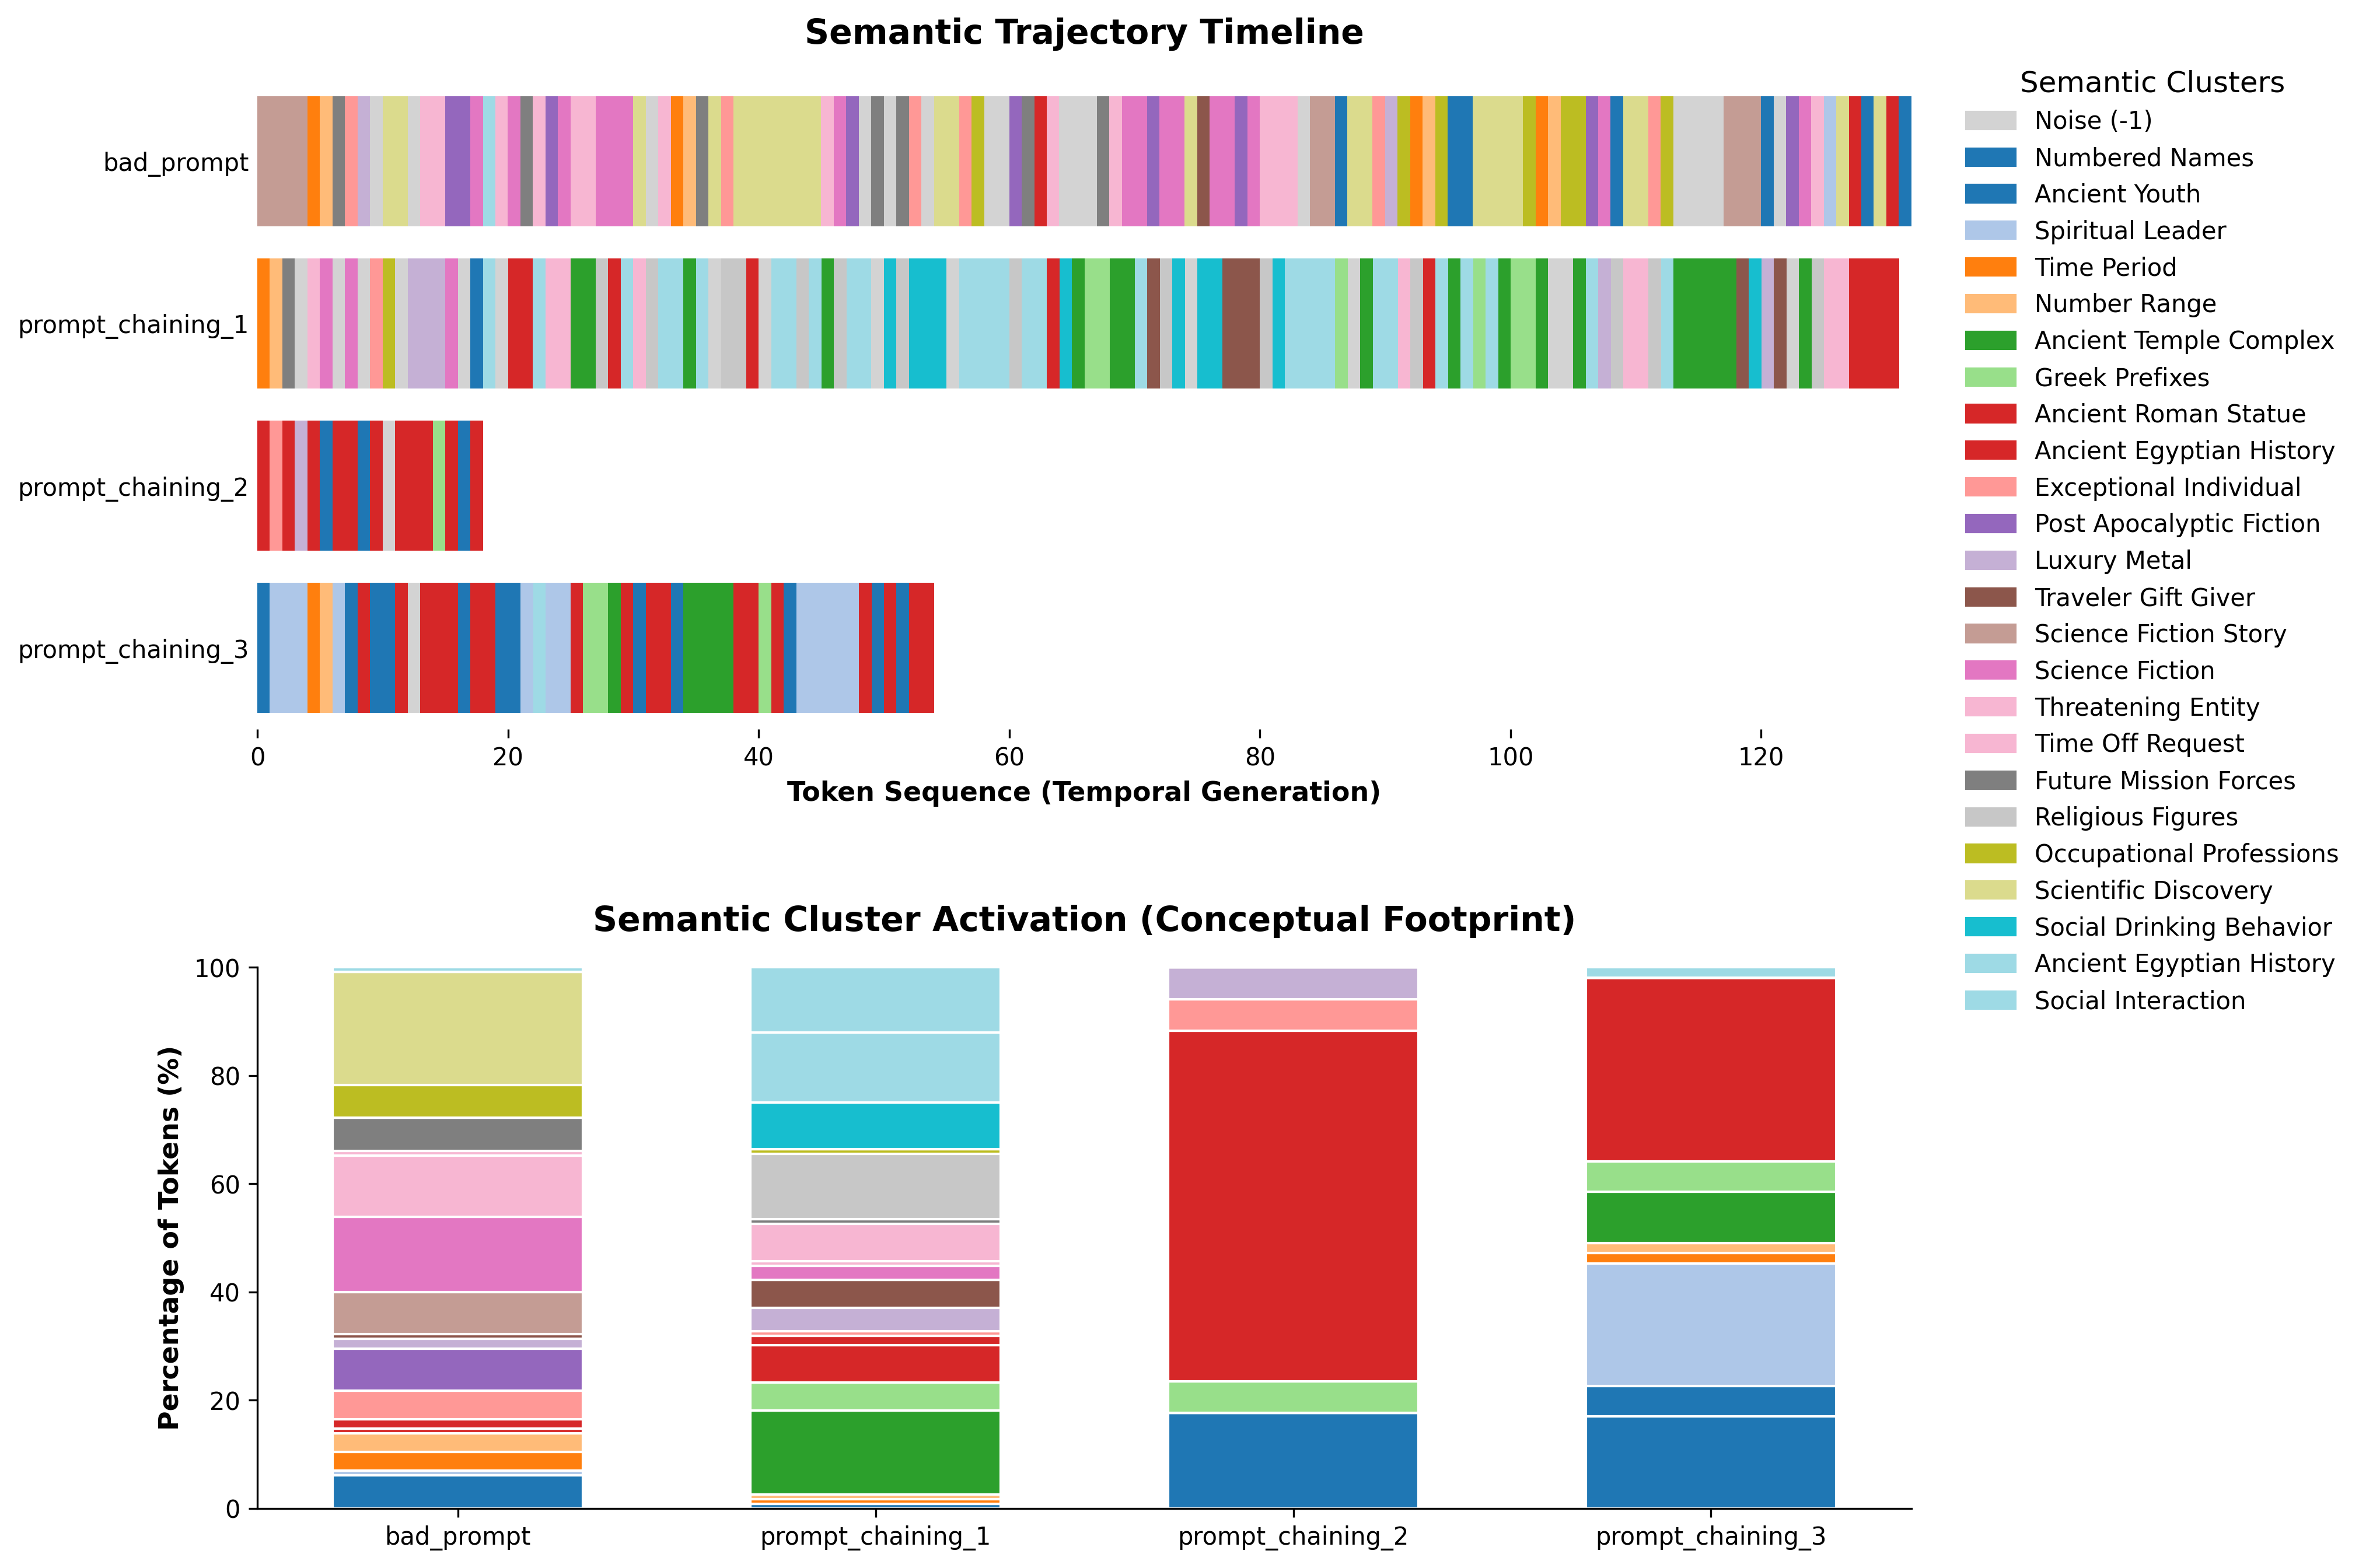
\includegraphics[width=1\textwidth]{assets/prompt-chaining_cluster_activation.png}    
    \caption{Cluster Activation nel Prompt Chaining. I grafici mostrano la variazione del focus semantico tra le fasi della catena.}
    \label{fig:act_chaining}
\end{figure}

\begin{figure}[htbp]
    \centering
    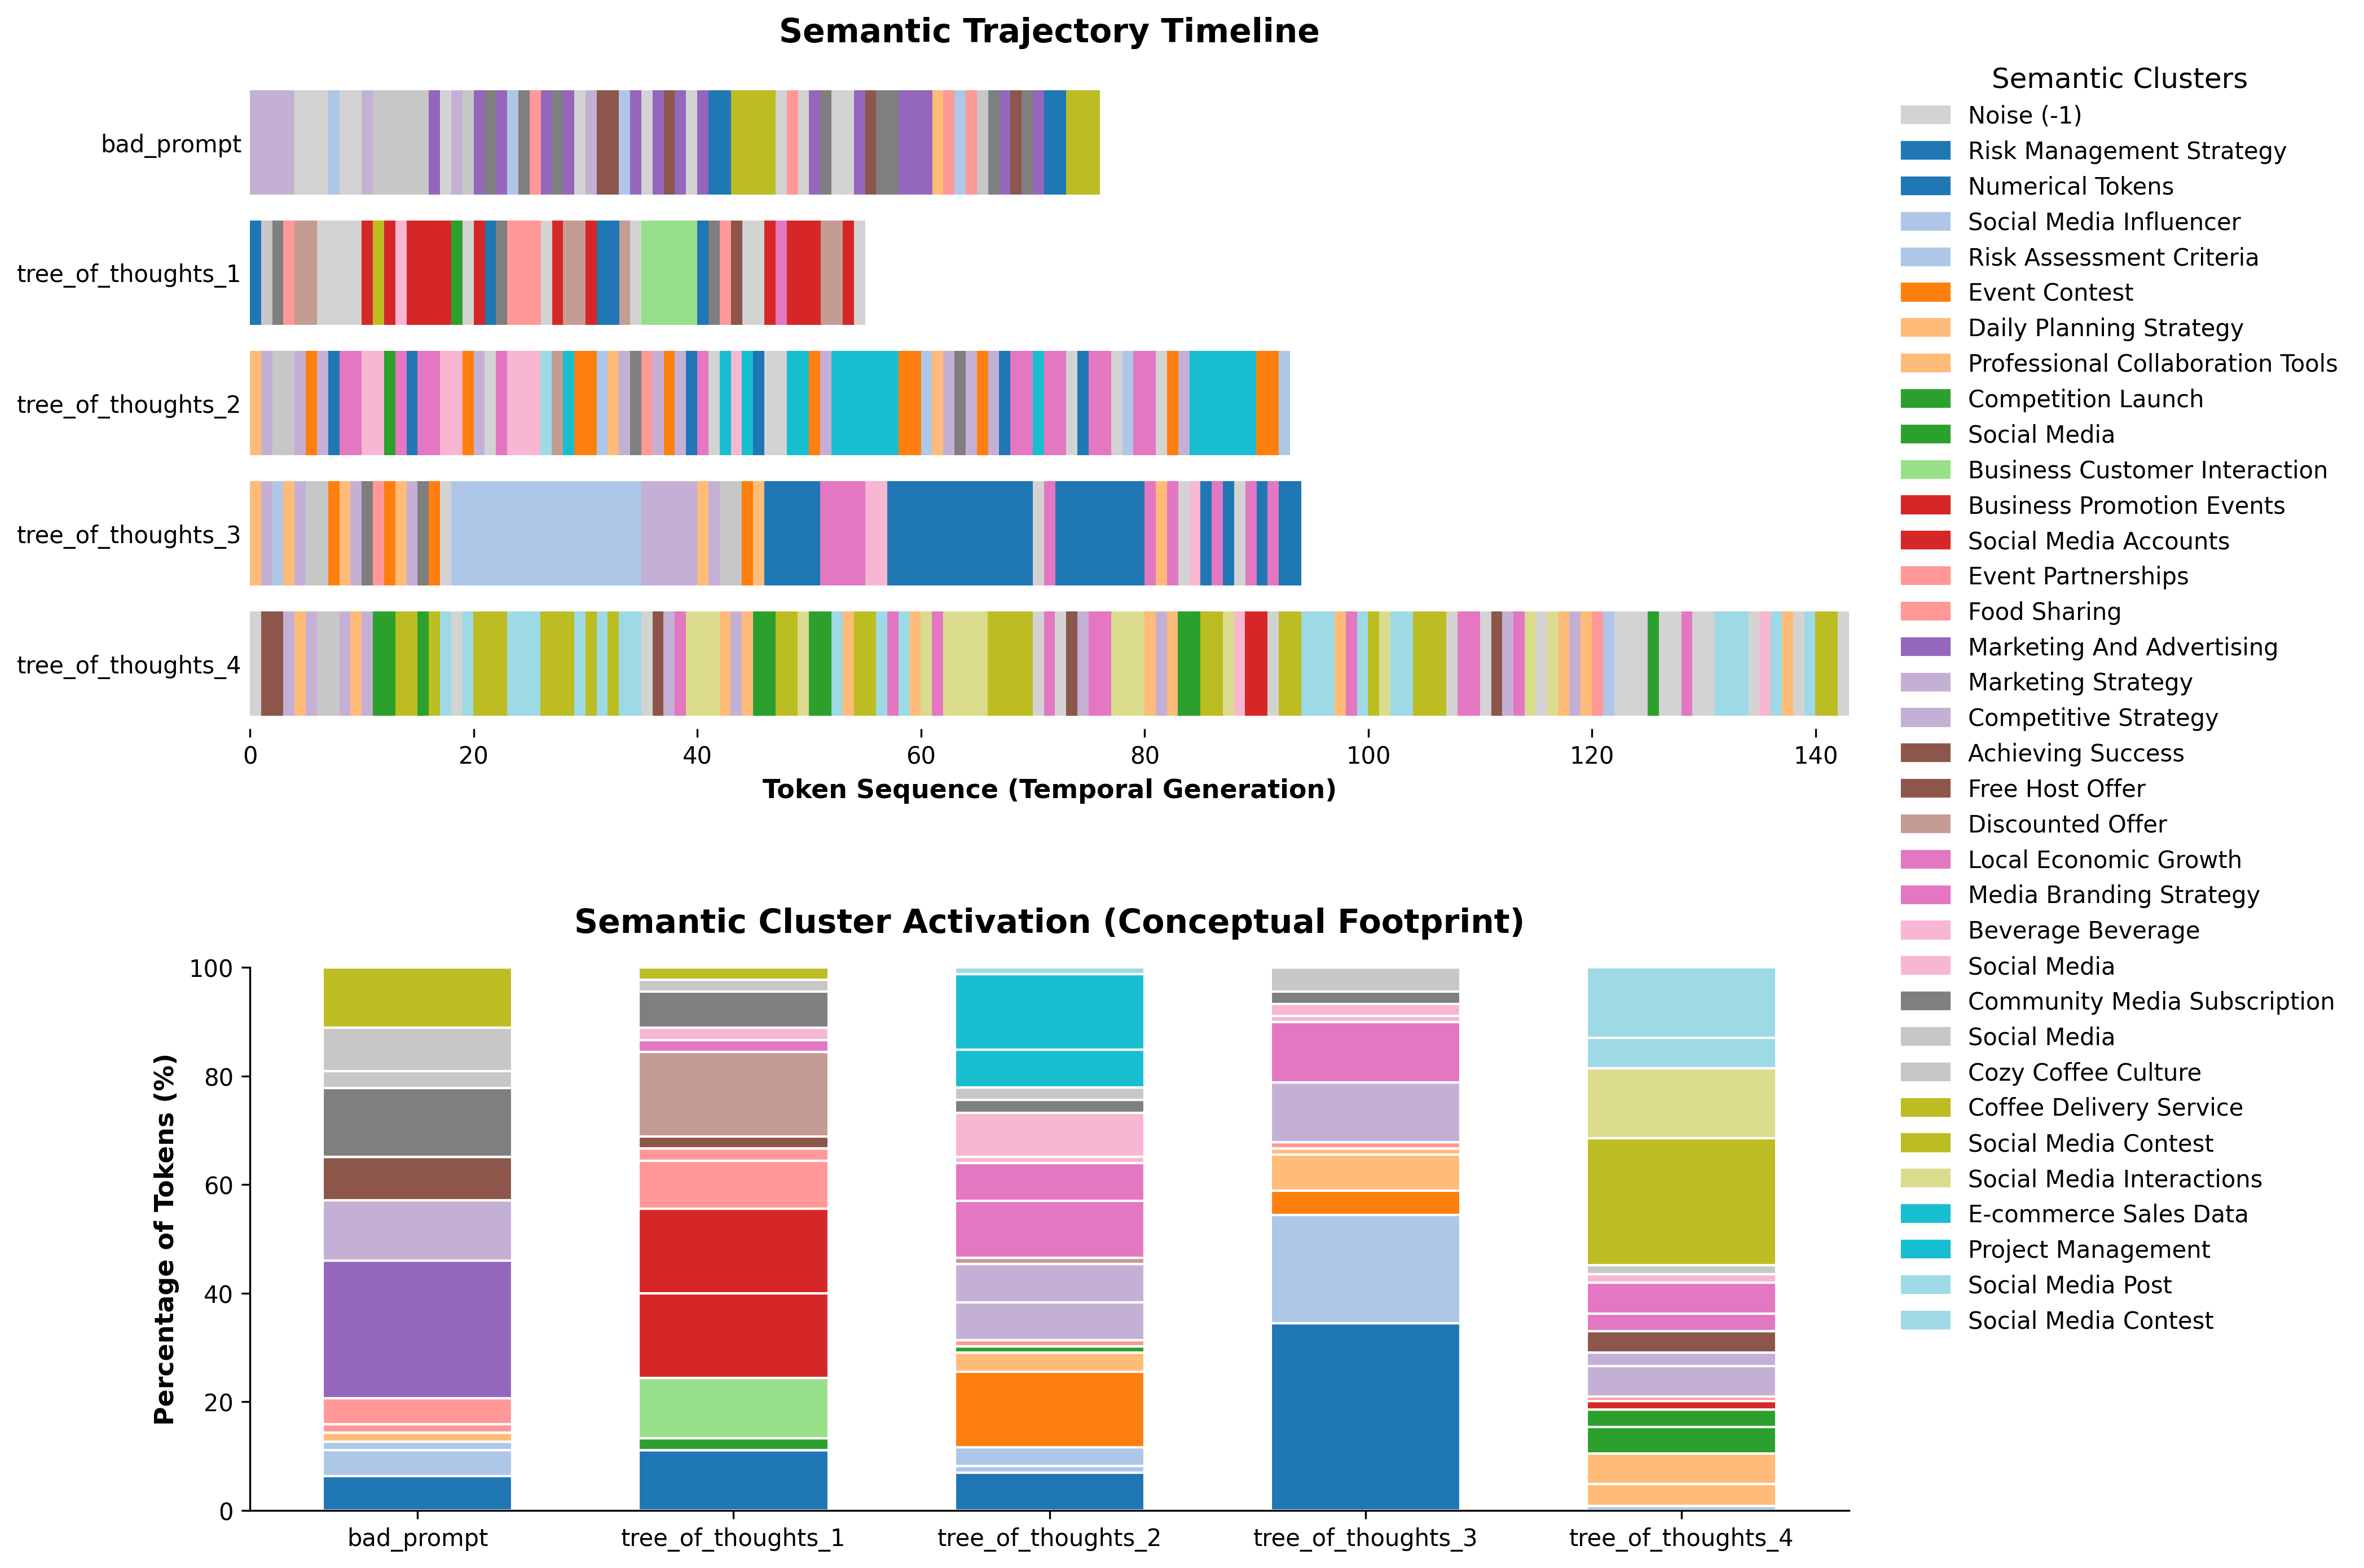
\includegraphics[width=1\textwidth]{assets/tree-of-thoughts_cluster_activation.png}
    \caption{Cluster Activation nel Tree of Thoughts. I diversi rami dell'albero esplorano set di cluster parzialmente disgiunti.}
    \label{fig:act_tot}
\end{figure}

Il prompt di base, che richiede di svolgere tre compiti simultaneamente, mostra un'attivazione distribuita su un numero più elevato di cluster. Frammentando la richiesta, le singole fasi tendono a concentrarsi su specifiche aree semantiche (Figura \ref{fig:act_chaining}). Ad esempio, la seconda fase (\textit{Chaining 2}, dedicata all'estrazione dei personaggi) concentra circa il 65\% della generazione su un singolo cluster (Cluster 8), per poi ridistribuirsi nella terza fase relativa alla creazione del quiz. La tecnica modula quindi la generazione facendola transitare attraverso stati semantici successivi, coerentemente con la divisione dei sottocompiti.

\newpage

\paragraph{Distribuzione Ramificata: Tree of Thoughts}
Il Tree of Thoughts estende la dinamica osservata nel Chaining. L'articolazione in rami decisionali (brainstorming, analisi, valutazione comparativa e pianificazione) comporta una distribuzione maggiormente articolata sullo spazio latente.



L'osservazione della Figura \ref{fig:act_tot} mostra come i diversi passaggi dell'albero decisionale tendano ad attivare regioni semantiche variabili. Il primo passaggio (\textit{ToT 1}) distribuisce i token principalmente su tre cluster (10, 11 e 19, ciascuno al 15.5\%); avanzando verso la fase di scelta strategica (\textit{ToT 3}), l'attivazione maggiore si registra sul Cluster 0 (34.4\%); infine, la fase di pianificazione (\textit{ToT 4}) coinvolge ulteriori domini, come il Cluster 28 (23.3\%). Questa variazione dei cluster attivi suggerisce che la struttura ad albero induca il modello a esplorare una pluralità di domini valutativi, ampliando l'eterogeneità concettuale rispetto a un prompt monolitico.